\section{Iteration 2: Binary IR vs. Valued IR}

With our first study, we have learned that with {\em coarse selection}, we can reduce the overall target selection time because in many cases there will be only one target in range and {\em fine selection} is not needed, and in cases where it's needed, the list length has been effectively reduced. However, in a dense environment, there could be more cases when disambiguation is needed. 

From Figure~\ref{fig:selection-time}B, the average results when disambiguation is involved is significantly increase. We challenge ourselves that ``can we do a better job in a dense environment?''

Previously we are only using IR reception as a signal for potential target identification. It's a binary result indicating that whether a target has received IR signal or not. But actually the IR intensity at the receiver side can provide more information than just the binary reception. The illuminance falls when the distance increases as well as when the angle inceases.
We have emprically measured the intensity distribution at the receiver side, and it's shown in Figure~\ref{fig:measurement}.

\begin{figure}[t]
\centering
\includegraphics[width=0.9\columnwidth]{figures/placeholder.pdf}
\caption{placeholder for emperical measurement.}
\label{fig:measurement}
\end{figure}


The intensity information is used in two ways:
\begin{enumerate}
\item When multiple targets have received IR signal and reported the intensity readings, we discard those whose intensities are significantly lower than the largest reading\footnote{In our current implementation, we empirically set it to be half, which is frequently used because it indicates a 3dB loss in the signal strength.}. In this case, when Binary IR doens't need disambiguation, the new design still doesn't need it. When the environment turns denser, the new design can filter some peripheral targets out, making the chances of entering disambiguation lower.
\item When disambiguation is still needed, we use the IR intensity as an indication of likelihood to sort the list. This will help us reduce the $t_{disambiguation}$ significantly if the first one appears matches the actual target. Given the imprecision of head orientation, this can hardly be always perfect.
\end{enumerate}

Though apparently with more information, we should be able to reduce the selection time. But the question we seek to answer is to further quantify such gain. We then performed another user study to compare the {\em Binary IR} and {\em Valued IR} designs.

For this study, since we are aiming at a denser environment, though we keep the node number to 10, but the environment setup has changed (see Figure~\ref{fig:study-layout2}). In total, we have XX users for this study \ben{more information about users later.} Each user performs the target acquisition study 30 times for each condition. Again half of them perform {\em Binary IR} first and the other half {\em Valued IR} first.

\begin{figure}[t]
\centering
\includegraphics[width=0.9\columnwidth]{figures/study-layout2.jpg}
\caption{The current environment setup \ben{needs annotation and a better photo.}.}
\label{fig:study-layout2}
\end{figure}

We then summarize the result of this study. 
\begin{enumerate}
\item Among the 150 trials in {\em Binary IR} condition, there are 104 times when disambiguation is needed. In {\em Valued IR} condition, only 65 out of 150 trials need disambiguation. We perform a Chi-square test on this result and the result is $\chi^2(1) = 20.611$, $p < 0.0001$. \ben{not sure about the degree of freedom being 1 here, will check later.} This demonstrates that the first intensity gain is from the reduction of chances when disambiguation is needed.
\item In the cases when disambiguation is needed, the {\em Valued IR} will sort the list based on the intensity reading. Indeed, out of the 65 times when disambiguation is involved, there are 38 (roughly 58\%) are right for {\em Valued IR}. However, for {\em Binary IR}, only 37 out of 104 (~35\%) are right. Again a Chi-square test demonstrates the statistical differences (with $\chi^2(1) = 8.487$, $p = 0.0036$. 
\end{enumerate}

Such gain can be seen from Figure~\ref{fig:study2} where the overall target acquisition time is obtained. The average time is 4.32 seconds and 3.71 second for {\em Binary IR} and {\em Valued IR}, respectively; and a t-test shows that they are also significantly different $t(282)=2.0922$, $p=0.03$.

\begin{figure}[t]
\centering
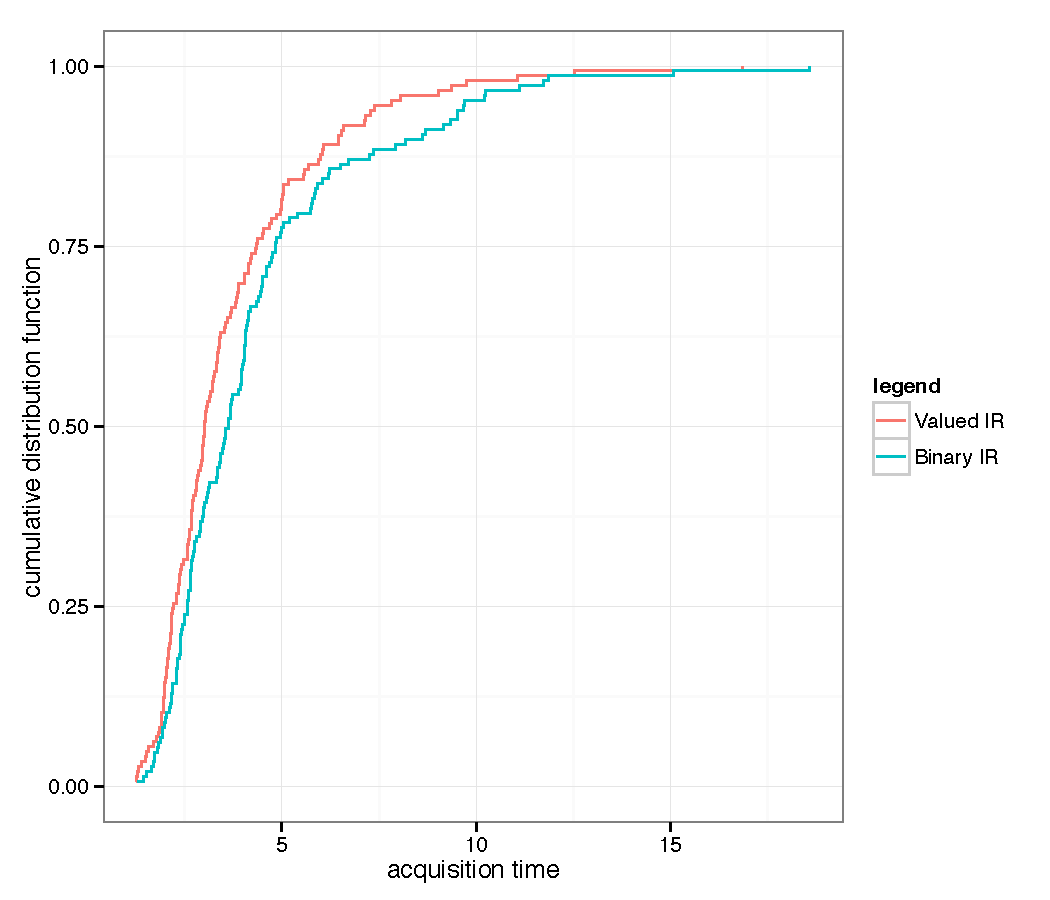
\includegraphics[width=0.9\columnwidth]{figures/study2_time.pdf}
\caption{The target acquisition of in {\em Valued IR} and {\em Binary IR} condition.}
\label{fig:study2}
\end{figure}

However, one side effect that we have abserved in this approach is that the {\em Valued IR} sometimes eliminates the right target during the filter stage. The rate is not that high (16 out of 150 cases, ~90\%), but this is the price to pay for a quicker average in this smarter system.

%%% Local Variables: 
%%% mode: latex
%%% TeX-master: "uist14"
%%% End: 
